\section{Resultados}

\subsection{Criterio de Parada}
Realizamos, para cada método, las mediciones comentadas en la sección anterior, obteniendo los siguientes resultados.
\begin{figure}[H]
  \centering
    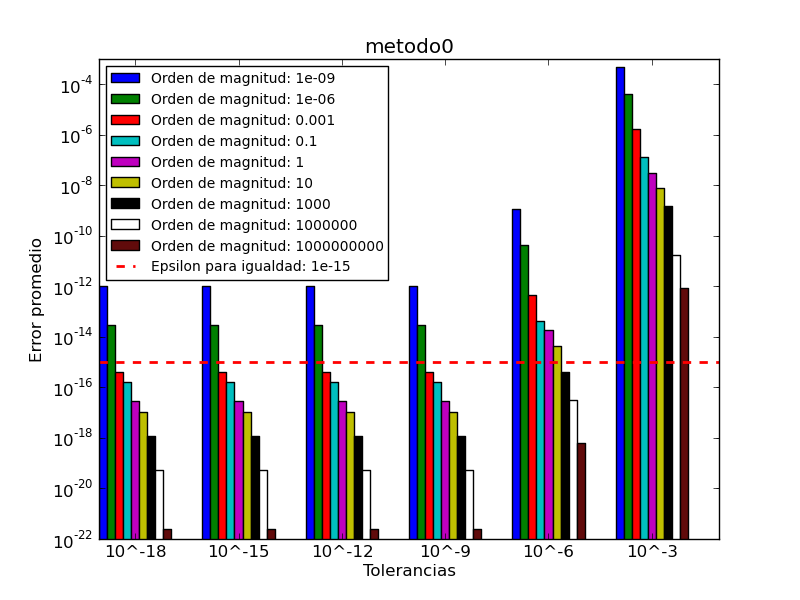
\includegraphics[width=0.9\textwidth]{../data/metodo0.png}
    \caption{Error relativo final para distintos valores de tolerancia en el criterio de parada utilizando el cero de $x^2-\alpha$ con el método de Newton para cada orden de magnitud medido.}
    \label{paradaMet0}
\end{figure}

Para el primer método, calculamos $z^{-1}$, siendo $z$ un cero de $f(x) = x^2-\alpha$ que obtuvimos mediante el método de Newton. En la figura \ref{paradaMet0} vemos el error relativo final (luego de calculado el cociente) según las distintas tolerancias. Observamos, por un lado, que todos los errores decrecen (no estrictamente) a medida que decrece la tolerancia, lo cual es esperable. Por otro lado, observamos un estancamiento del error para $\tau < 10^{-9}$, con lo cual éste será el valor elegido para este método. Si bien es llamativo que el error no se reduzca para tolerancias menores, sabiendo que el método converge cuadráticamente podemos pensar que el error relativo del criterio de parada se reduce, en una iteración de un valor en el orden de $10^-6$ a uno por debajo de $10^-18$, haciendo que el método termine para todas las tolerancias intermedias al mismo tiempo. Pensamos en investigar qué sucedería para tolerancias menores, pero dado que consideramos como iguales valores que difieran en menos de $10^{-15}$ consideramos que no tenía significación.

Observemos también que el error relativo se hace más significativo cuanto menor es el orden de magnitud, lo que indicaría que el error absoluto no necesariamente acompaña la magnitud de $\alpha$. Atribuimos esto a errores numéricos, que se introducen siempre independientemente del valor representado.


\begin{figure}[H]
  \centering
    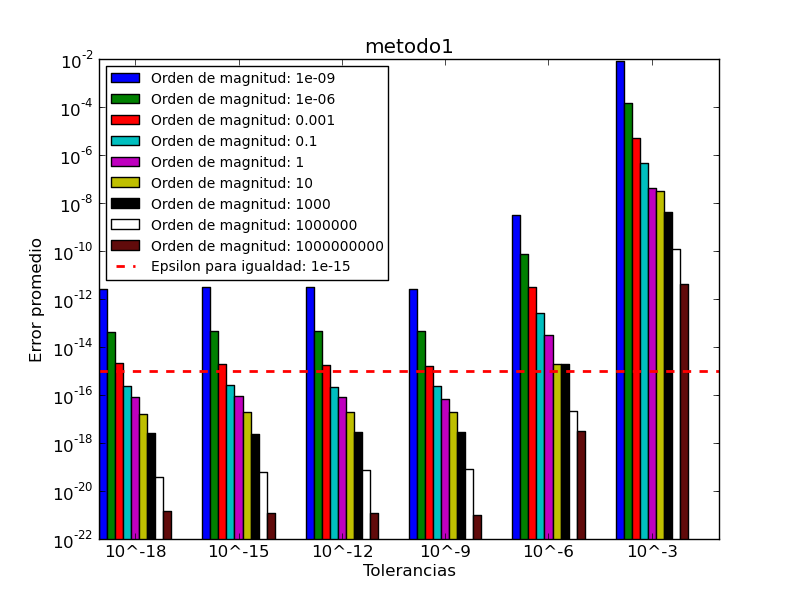
\includegraphics[width=0.9\textwidth]{../data/metodo1.png}
    \caption{Error relativo final para distintos valores de tolerancia en el criterio de parada para el cero de $\frac{1}{x^2} - \alpha$ con el método de Newton para cada orden de magnitud medido.}
    \label{paradaMet1}
\end{figure}

Observemos que el gráfico es muy similar al de la figura \ref{paradaMet1}, con lo cual, al tratarse del mismo método, caben argumentos similares: el decrecimiento y estancamiento lo atribuimos a la rapidez con la que converge el método y podemos utilizar $10^{-9}$ para el criterio de parada.

\begin{figure}[H]
  \centering
    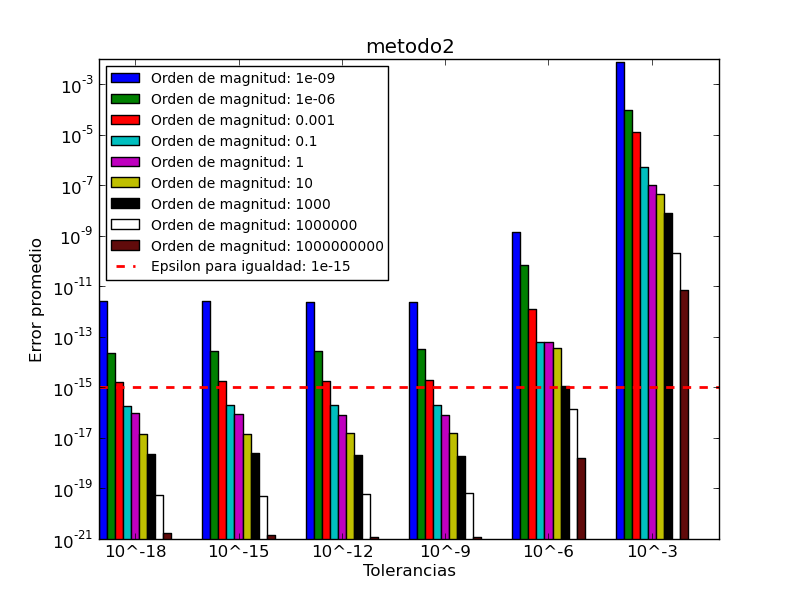
\includegraphics[width=0.9\textwidth]{../data/metodo2.png}
    \caption{Error relativo final para distintos valores de tolerancia en el criterio de parada para el cero de $\frac{1}{x^2} - \alpha$ con el método de punto fijo para $\frac{1}{\alpha x} + \frac{x - \alpha x^3}{2}$, para cada orden de magnitud medido.}
    \label{paradaMet2}
\end{figure}

Al igual que en el caso anterior, la figura \ref{paradaMet2}, al tratarse de un método cuadrático, admite un análisis análogo a los casos anteriores. En este caso también elegiremos $10^{-9}$.

\begin{figure}[H]
  \centering
    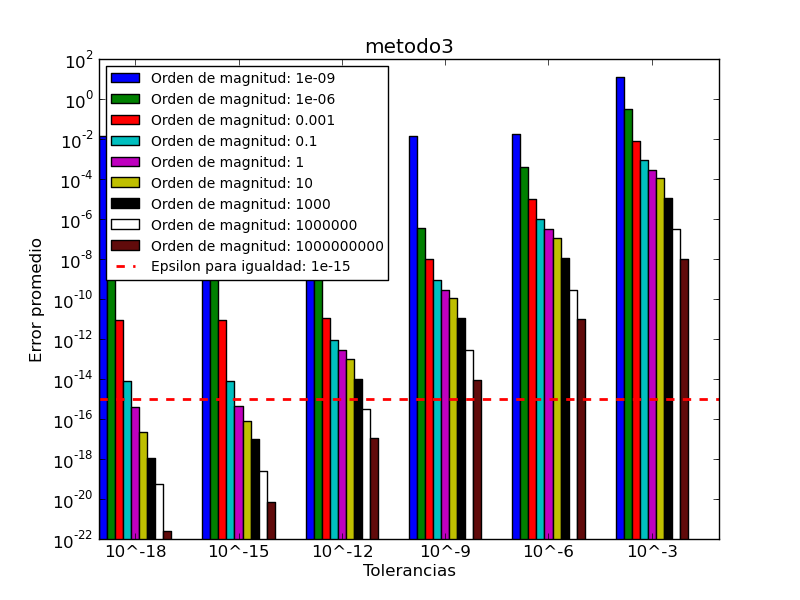
\includegraphics[width=0.9\textwidth]{../data/metodo3.png}
    \caption{Error relativo final para distintos valores de tolerancia en el criterio de parada obteniendo el cero de $x^2 - \alpha$ mediante bisección, para cada orden de magnitud medido.}
    \label{paradaMet3}
\end{figure}

Como dijimos, no esperábamos grandes resultados para este método. Elegiremos para seguir $10^{-15}$, que es donde se detiene la reducción del error (nuevamente, relacionado con el criterio de igualdad establecido). Vemos que para los órdenes más pequeños el error relativo es significativo, aún para las tolerancias menores, lo que indica que el error absoluto sigue siendo importante. Sabemos que para $\sqrt{\alpha}$ éste está acotado por la mitad de la longitud del intervalo en el último paso de bisección, pero al calcularle el recíproco, tratándose de valores pequeños, éste crece considerablemente.



